\documentclass[11pt,a4paper]{article}

\usepackage{fontspec}
\usepackage{polyglossia}
\setdefaultlanguage{russian}
\setotherlanguage{english}
\setmainfont{Times New Roman}
\setsansfont{Arial}
\setmonofont{Courier New}
\newfontfamily\cyrillicfont{Times New Roman}
\newfontfamily\cyrillicfontsf{Arial}
\newfontfamily\cyrillicfonttt{Courier New}

\usepackage[a4paper,margin=2.25cm]{geometry}
\usepackage{amsmath,amssymb,mathtools}
\usepackage{booktabs}
\usepackage{graphicx}
\usepackage{caption}
\usepackage{subcaption}
\usepackage{xcolor}
\usepackage{hyperref}
\usepackage[numbers,sort&compress]{natbib}

\setlength{\emergencystretch}{3em}

\hypersetup{
  colorlinks=true,
  linkcolor=blue!45!black,
  citecolor=blue!45!black,
  urlcolor=blue!45!black
}

\newcommand{\R}{\mathbb{R}}
\newcommand{\1}{\mathbf{1}}
\newcommand{\argmin}{\operatorname*{arg\,min}}
\newcommand{\inner}[2]{\left\langle #1,#2\right\rangle}
\newcommand{\norm}[1]{\left\lVert #1\right\rVert}

\title{\textbf{Decentralized Block-Coordinate Frank-Wolfe для semi-relaxed OT color transfer}}
\author{Экспериментальный сетап репозитория \texttt{dbcfw\_timevarying\_benchmark}}
\date{22 июня 2026}

\begin{document}
\maketitle

\begin{abstract}
В документе описан новый экспериментальный сетап для задачи переноса цветовой палитры через semi-relaxed optimal transport. Мы берем постановку semi-relaxed OT, в которой одна маргиналь сохраняется точно, а другая штрафуется квадратично, и поднимаем ее в децентрализованный режим. Сравниваются два децентрализованных projection-free метода: DFW как полный Frank-Wolfe шаг по всем столбцам транспортного плана и DBCFW как блочный Frank-Wolfe шаг по одному столбцу. Основной результат: при одинаковом oracle budget DBCFW достигает меньшего objective residual, меньшего Frank-Wolfe duality gap и более точной транспортной матрицы относительно сильного централизованного BCFW reference. Это честное сравнение по числу вызовов линейного оракула, но не по числу коммуникационных раундов.
\end{abstract}

\section{Контекст и литература}

Классический optimal transport (OT) сравнивает распределения через стоимость переноса массы. В дискретной форме эта задача восходит к линейной программе Канторовича и является стандартным инструментом для вычислительной математики, imaging и machine learning; см. обзор \citet{peyre2019computational}. Для color transfer OT естественен: цвета изображения представляются как распределение в RGB-пространстве, а транспортный план задает, как цвета исходного изображения переводятся в цвета целевого. Relaxed и regularized OT для цветовых преобразований обсуждаются, например, у \citet{ferradans2014regularized}.

Frank-Wolfe, или conditional gradient, был предложен \citet{frank1956algorithm} как projection-free метод для гладкой выпуклой оптимизации на компактных выпуклых множествах. Современная интерпретация через linear minimization oracle (LMO) и duality gap дана в \citet{jaggi2013revisiting}. Для задач с блочно-разделимыми ограничениями естественен BCFW: обновляется не весь объект, а один блок или батч блоков. Такая идея систематически изучалась, в частности, у \citet{lacostejulien2013block}. Для децентрализованного режима используется линия работ о decentralized FW и consensus/tracking механизмах, например \citet{wai2017decentralized}.

Ближайшая к нашему OT-сетапу работа - статья \citet{fukunaga2021fast}. Авторы рассматривают fast BCFW для semi-relaxed OT, показывают связь linearization duality gap с лагранжевым gap и демонстрируют эффективность на color transfer. В нашем эксперименте центральная идея той статьи переносится в децентрализованный запуск: мы сравниваем не только FW против BCFW, а DFW против DBCFW в одном и том же distributed graph setup.

\section{Математическая постановка}

Пусть исходное изображение аппроксимировано палитрой
\[
  \mu_s = \sum_{i=1}^{m} a_i \delta_{x_i},
  \qquad
  a \in \Delta_m,\quad x_i \in \R^3,
\]
а целевое изображение - палитрой
\[
  \mu_t = \sum_{j=1}^{n} b_j \delta_{y_j},
  \qquad
  b \in \Delta_n,\quad y_j \in \R^3.
\]
В эксперименте $m=n=32$, а центры $x_i,y_j$ получаются k-means кластеризацией пикселей в RGB-пространстве. Стоимость переноса задается матрицей
\[
  C_{ij} = \norm{x_i-y_j}_2^2.
\]

Balanced OT решает линейную программу
\[
  \min_{T \ge 0} \inner{C}{T}
  \quad \text{s.t.} \quad
  T\1_n=a,\quad T^\top\1_m=b,
\]
где $T_{ij}$ - масса, отправленная из исходного цвета $x_i$ в целевой цвет $y_j$. Для изображений жесткое сохранение обеих маргиналей может быть слишком ограничительным: палитры могут иметь разные массы и разную выраженность цветовых мод. Поэтому используется semi-relaxed OT:
\begin{equation}
\label{eq:semi-relaxed}
  \min_{T\in\mathcal{D}_b}
  f(T)
  =
  \inner{C}{T}
  +
  \frac{1}{2\lambda}\norm{T\1_n-a}_2^2,
  \qquad
  \mathcal{D}_b=\{T\in\R_+^{m\times n}:T^\top\1_m=b\}.
\end{equation}
Параметр $\lambda>0$ управляет силой штрафа за нарушение исходной маргинали. Чем меньше $\lambda$, тем ближе задача к balanced OT по строкам; чем больше $\lambda$, тем свободнее источник может менять массы.

Градиент цели имеет простой вид:
\begin{equation}
\label{eq:gradient}
  \nabla f(T) = C + \frac{1}{\lambda}(T\1_n-a)\1_n^\top.
\end{equation}
Ограничение $\mathcal{D}_b$ разделяется по столбцам: каждый столбец $T_{:j}$ лежит в scaled simplex
\[
  \{u\in\R_+^m:\1_m^\top u=b_j\}.
\]
Поэтому LMO для FW раскладывается на независимые столбцовые задачи. Для заданного градиента $G$:
\begin{equation}
\label{eq:lmo}
  S(G)_{:j}= b_j e_{i_j},
  \qquad
  i_j \in \argmin_{i\in\{1,\ldots,m\}} G_{ij}.
\end{equation}
Именно эта структура делает BCFW особенно подходящим для semi-relaxed OT: один блочный шаг обновляет один или несколько столбцов транспортного плана, не решая большую проекционную задачу.

Для контроля сходимости используется стандартный Frank-Wolfe gap:
\begin{equation}
\label{eq:gap}
  g(T)
  =
  \inner{T-S(\nabla f(T))}{\nabla f(T)}.
\end{equation}
Для выпуклой гладкой задачи это не просто эвристика: $g(T)$ является вычислимым сертификатом субоптимальности, то есть $f(T)-f(T^\star)\le g(T)$ при точном LMO.

\section{Как транспортный план дает color transfer}

После оптимизации план $T$ переводится в стохастическую строковую матрицу
\[
  P_{ij}
  =
  \frac{T_{ij}}{\sum_{\ell=1}^{n} T_{i\ell}}
  \quad
  \text{если } \sum_{\ell}T_{i\ell}>0.
\]
Затем каждый исходный цвет $x_i$ заменяется барицентрическим целевым цветом
\[
  \hat{x}_i = \sum_{j=1}^{n} P_{ij}y_j.
\]
Пиксель исходного изображения сначала получает label ближайшего palette center $x_i$, после чего перекрашивается в $\hat{x}_i$. Поэтому ошибка транспортной матрицы относительно reference важнее, чем только визуальное впечатление: если $T$ близок к reference, то и row-normalized mapping ближе к желаемому OT color map.

\section{Сравниваемые методы}

\paragraph{FW.}
Centralized FW на каждой итерации считает полный градиент, решает LMO по всем $n$ столбцам и делает шаг
\[
  T_{k+1}=(1-\gamma_k)T_k+\gamma_k S(\nabla f(T_k)).
\]
В нашем децентрализованном сравнении прямым аналогом является DFW: каждый агент делает полный FW-шаг по всем столбцам, а затем состояние и gradient tracker смешиваются по графу.

\paragraph{BCFW.}
BCFW выбирает блок $B_k\subset\{1,\ldots,n\}$ и решает LMO только по этим столбцам:
\[
  D_{:j}=S(\nabla f(T_k))_{:j}-T_{k,:j},\quad j\in B_k,
  \qquad
  D_{:j}=0,\quad j\notin B_k.
\]
После этого выполняется line search по направлению $D$. При $B_k=\{1,\ldots,n\}$ получаем обычный FW. При $|B_k|=1$ получаем максимально блочный режим, который особенно дешев по LMO, но требует больше итераций.

\paragraph{DFW.}
В децентрализованном режиме есть $N$ агентов. Агент $p$ хранит свой план $T_k^{(p)}$ и локальный gradient tracker. На каждом раунде применяется doubly stochastic mixing matrix $W_k$, соответствующая текущему коммуникационному графу:
\[
  \bar{T}_k^{(p)}=\sum_{q=1}^N W_{k,pq}T_k^{(q)}.
\]
После смешивания агент строит FW-направление по всем столбцам. В нашем коде DFW реализуется как тот же decentralized routine, но с batch size $n$.

\paragraph{DBCFW.}
DBCFW использует тот же граф, тот же tracker и тот же line-search механизм, но обновляет малый набор столбцов. В reported run используется batch size $1$:
\[
  |B_k^{(p)}|=1.
\]
То есть каждый агент за один раунд решает только один столбцовый LMO, а весь прогресс на уровне полного плана набирается частыми локальными шагами. Это и есть наш децентрализованный блочно-координатный перенос идеи BCFW на semi-relaxed OT.

\section{Экспериментальный дизайн}

Основной color-transfer запуск:
\begin{center}
\begin{tabular}{ll}
\toprule
Параметр & Значение \\
\midrule
Source / target & \texttt{rocket} $\to$ \texttt{coffee} \\
Число цветов & $m=n=32$ \\
Агенты & $N=8$ \\
Relaxation & $\lambda=0.08$ \\
Graph & Erdos-Renyi connected, edge probability $0.45$ \\
Seed / graph seed & $202$ / $1202$ \\
Cost noise & $0.0$ \\
Stepsize & exact line search along FW direction \\
Reference & centralized BCFW, $1000$ oracle epochs \\
Budget for DFW/DBCFW & $80$ oracle epochs \\
\bottomrule
\end{tabular}
\end{center}

Reference нужен не как competing method, а как сильная аппроксимация $T^\star$ для метрик. Он строится централизованным BCFW с существенно большим бюджетом: $1000$ oracle epochs. Для DFW и DBCFW бюджет одинаков по числу LMO-column calls:
\[
  \text{oracle epochs}
  =
  \frac{\text{total LMO columns}}{Nn}.
\]
Это честная единица вычислительной работы, потому что и DFW, и DBCFW используют один и тот же столбцовый LMO \eqref{eq:lmo}; отличается только группировка этих вызовов по итерациям.

Важно: сравнение не является честным по коммуникациям. DFW делает $80$ communication rounds, а DBCFW - $2560$ rounds, потому что один полный DFW round обрабатывает $n=32$ столбца, а DBCFW обрабатывает один столбец за round. Поэтому основной вывод формулируется как oracle-efficiency win, а не communication-efficiency win.

\section{Метрики}

Мы используем четыре основные метрики:
\begin{enumerate}
  \item Objective residual к сильному reference:
  \[
    f(T_k)-f(T_{\mathrm{ref}}).
  \]
  Это показывает, насколько хорошо метод минимизирует именно semi-relaxed OT objective.

  \item Frank-Wolfe duality gap $g(T_k)$ из \eqref{eq:gap}. Это внутренний сертификат качества FW-типа методов.

  \item Ошибка транспортного плана:
  \[
    e_M(T_k)=
    \frac{\norm{T_k-T_{\mathrm{ref}}}_F}{\norm{T_{\mathrm{ref}}}_F}.
  \]
  Эта метрика важна для color transfer, потому что именно транспортный план задает mapping цветов.

  \item Variance of column gaps. Для столбца $j$ берется локальный вклад в FW gap:
  \[
    g_j(T)=\inner{T_{:j}-S(\nabla f(T))_{:j}}{\nabla f(T)_{:j}},
  \]
  и далее считается дисперсия по $j$. Низкая дисперсия означает, что метод не оставляет отдельные столбцы сильно недообработанными.
\end{enumerate}

\section{Результаты}

\begin{table}[h]
\centering
\caption{Финальные значения после $80$ oracle epochs. Меньше - лучше для всех метрик, кроме budget columns.}
\label{tab:results}
\begin{tabular}{lrrr}
\toprule
Метрика & DFW & DBCFW & Улучшение DBCFW \\
\midrule
$f(T)-f(T_{\mathrm{ref}})$ & $7.230\cdot 10^{-3}$ & $9.118\cdot 10^{-4}$ & $7.9\times$ ниже \\
FW duality gap & $1.282\cdot 10^{-2}$ & $1.077\cdot 10^{-3}$ & $11.9\times$ ниже \\
Transport matrix error & $2.027\cdot 10^{-1}$ & $5.498\cdot 10^{-2}$ & $3.7\times$ ниже \\
Column-gap variance & $1.147\cdot 10^{-7}$ & $1.325\cdot 10^{-9}$ & $86.5\times$ ниже \\
Communication rounds & $80$ & $2560$ & не win по коммуникациям \\
\bottomrule
\end{tabular}
\end{table}

Reference objective равен
\[
  f(T_{\mathrm{ref}})=0.054690,
  \qquad
  g(T_{\mathrm{ref}})=1.17\cdot 10^{-4}.
\]
После равного oracle budget DBCFW приходит к objective $0.055602$, тогда как DFW останавливается на $0.061919$. Разница не сводится к одному gap: DBCFW также заметно ближе к самой reference transport matrix.

\begin{figure}[p]
  \centering
  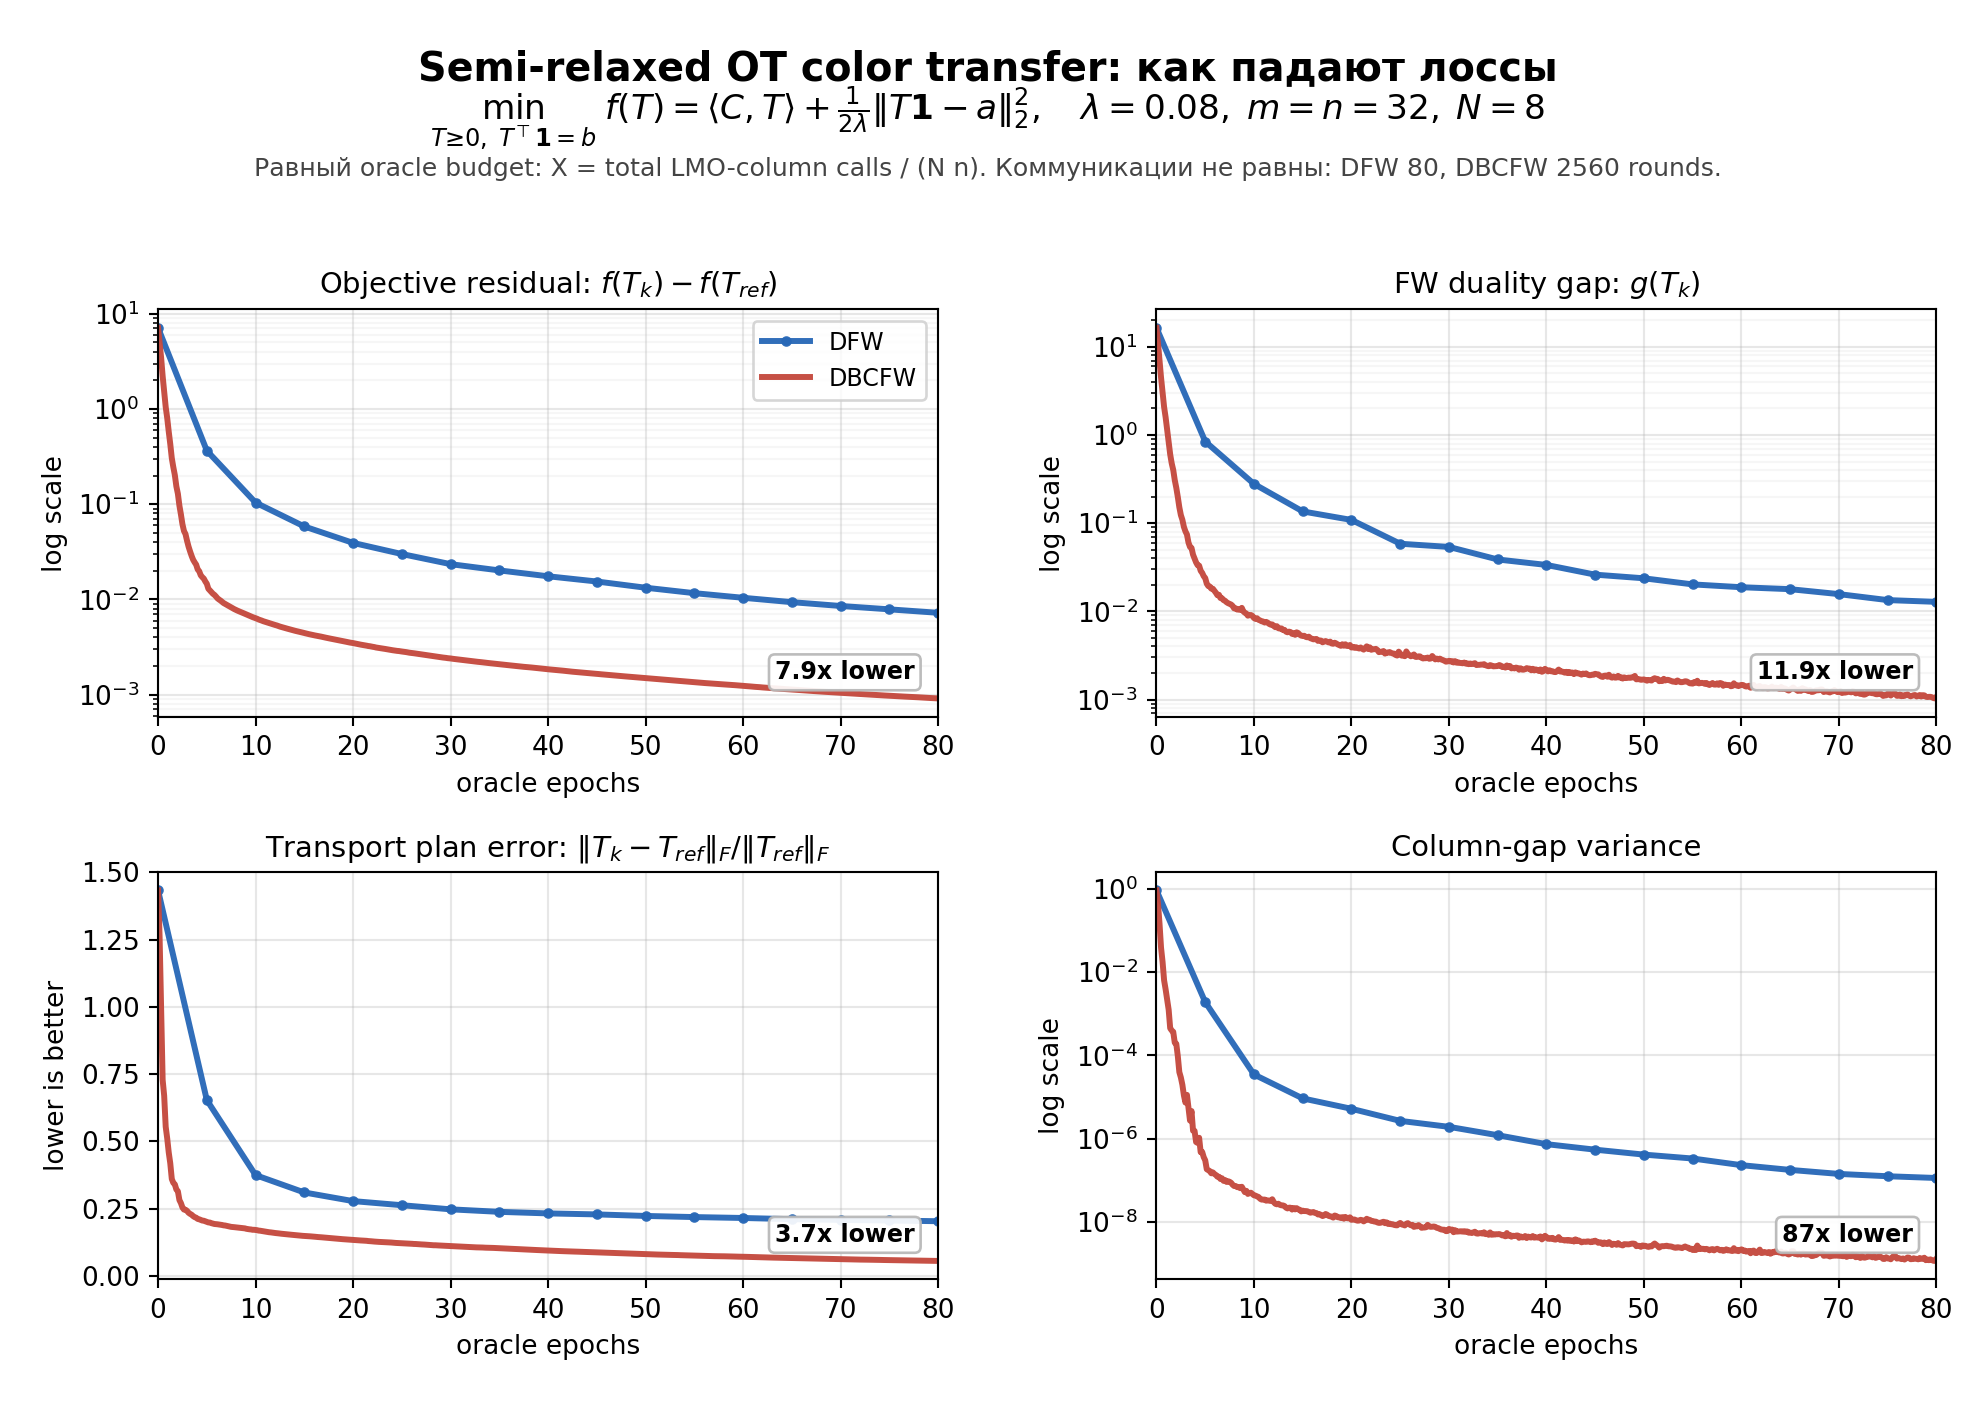
\includegraphics[width=\textwidth]{figures/mathematical_loss_curves_clean.png}
  \caption{Основной результат. При одинаковом числе LMO-column calls DBCFW быстрее снижает objective residual, FW duality gap, ошибку транспортного плана и variance of column gaps. Ось $x$ - oracle epochs, а не communication rounds.}
  \label{fig:main-loss}
\end{figure}

\begin{figure}[p]
  \centering
  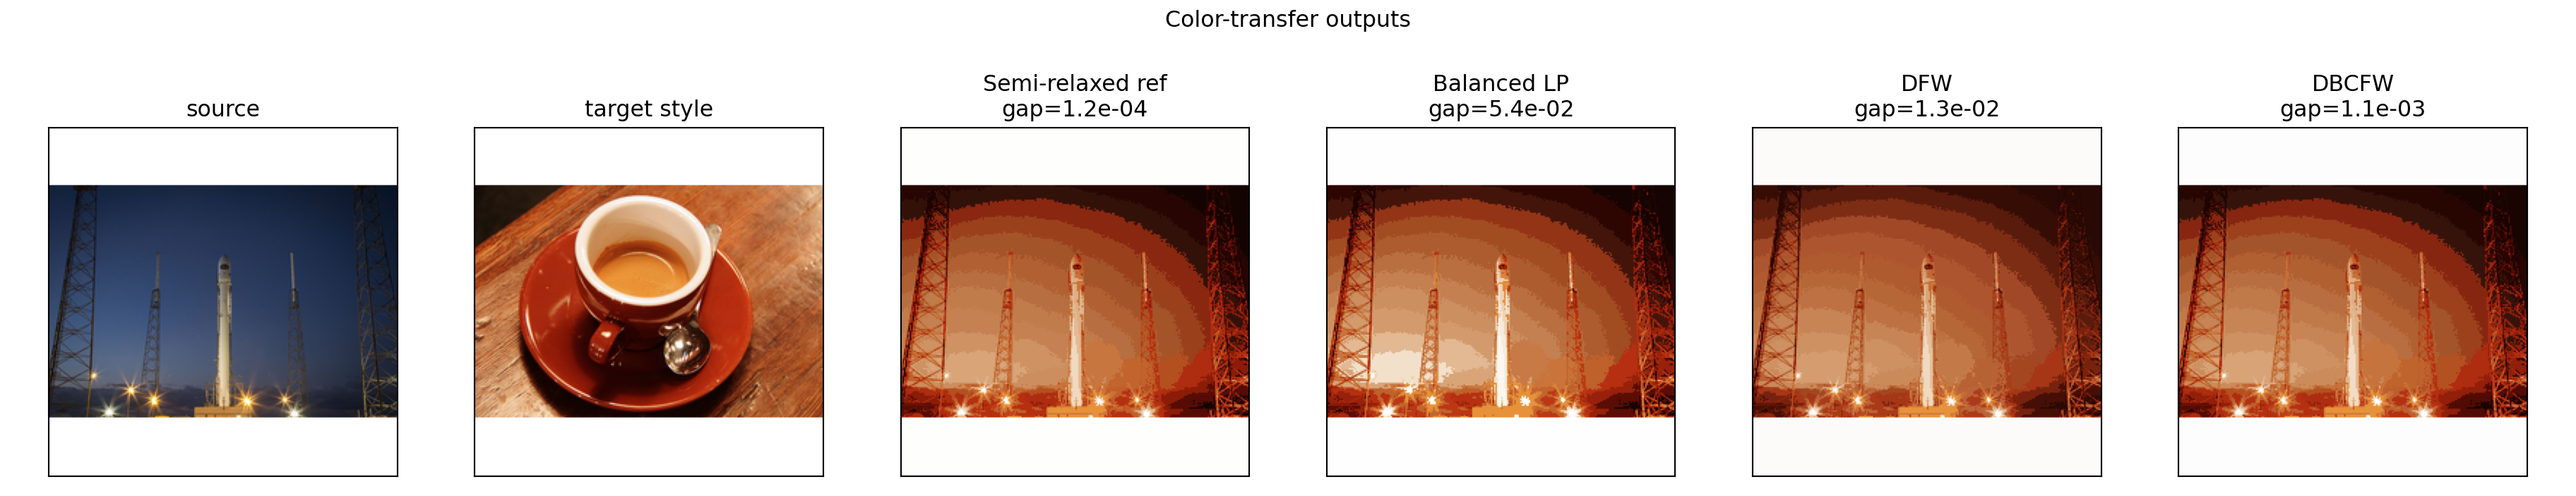
\includegraphics[width=\textwidth]{figures/color_transfer_comparison.png}
  \caption{Визуальная проверка color transfer. DBCFW ближе к semi-relaxed reference не только по objective/gap, но и по виду итогового переноса цветов.}
  \label{fig:visual}
\end{figure}

\begin{figure}[p]
  \centering
  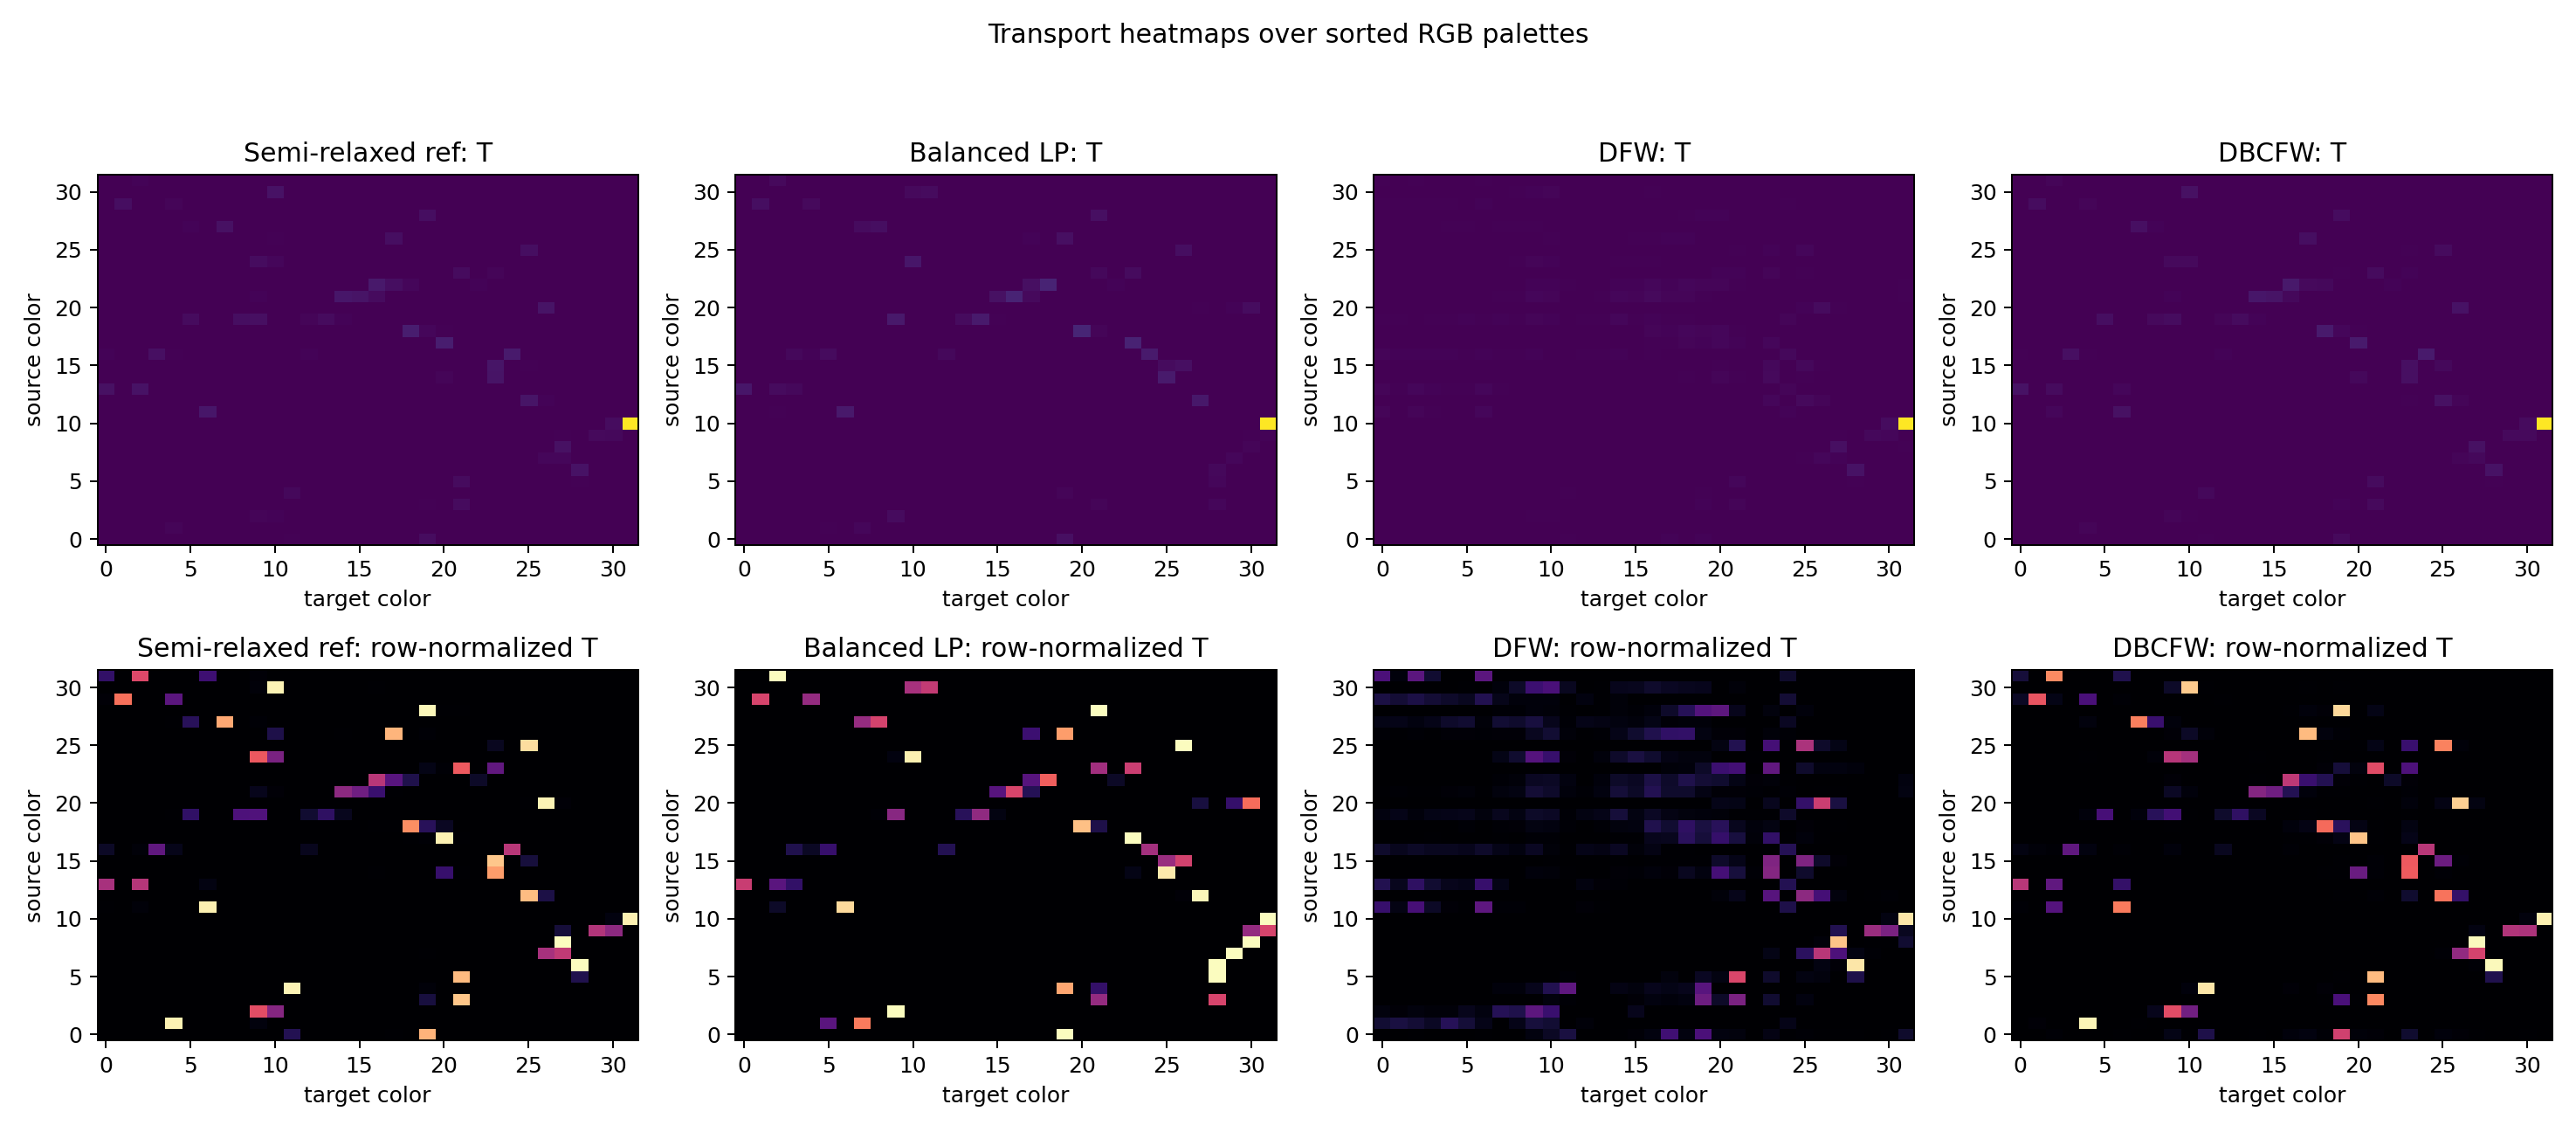
\includegraphics[width=\textwidth]{figures/palette_transport_heatmaps.png}
  \caption{Транспортные матрицы и row-normalized transport matrices. Для переноса цвета используется именно row-normalized версия плана.}
  \label{fig:heatmaps}
\end{figure}

\section{Почему DBCFW выигрывает в этом сетапе}

Главная причина - структура области $\mathcal{D}_b$. Ограничения по столбцам независимы, а LMO \eqref{eq:lmo} решается отдельно для каждого target color. В DFW полный шаг одновременно меняет все столбцы и использует один общий step size. Такой шаг может быть консервативным: хорошие направления для разных столбцов имеют разную локальную геометрию, но им приходится двигаться с общей $\gamma_k$.

DBCFW обновляет один столбец за раз. При равном числе LMO-column calls это означает большее число мелких descent/mixing steps. Каждый блочный шаг получает собственный line search, а column gaps быстрее выравниваются. Это видно по метрике column-gap variance: она у DBCFW ниже примерно в $86.5\times$. С практической точки зрения это означает, что метод не просто уменьшает глобальный gap, а равномернее дорабатывает transport plan по целевым цветам.

Второй фактор - близость задачи к блочной модели из \citet{fukunaga2021fast}. Их центральный результат состоит в том, что BCFW особенно полезен для semi-relaxed OT. Наш результат согласуется с этой картиной: когда semi-relaxed OT переносится в децентрализованный setup, блочная версия сохраняет преимущество по oracle-efficiency.

\section{Почему сравнение справедливое и где его границы}

Сравнение справедливое в следующем смысле:
\begin{itemize}
  \item одна и та же задача: те же изображения, палитры, cost matrix, $\lambda$, seed;
  \item один и тот же network setup: $N=8$, тот же Erdos-Renyi graph seed;
  \item одинаковая инициализация транспортного плана;
  \item одинаковый столбцовый LMO;
  \item одинаковый line search;
  \item одинаковый oracle budget: $80$ oracle epochs.
\end{itemize}

Сравнение не справедливое по communication rounds, и это сознательно отражено в подписи к Figure~\ref{fig:main-loss}. Если в приложении главным ресурсом является связь, нужно дополнительно сравнивать кривые против communication rounds или wall-clock time. В текущем документе утверждение такое: DBCFW лучше по oracle budget для semi-relaxed OT color transfer. Это не утверждение о меньшей коммуникационной цене.

\section{Как воспроизвести}

Запуск, соответствующий сохраненным результатам:
\begin{verbatim}
cd experiments/dbcfw_timevarying_benchmark
python -m dbcfw_bench.cli ot-color-transfer \
  --source rocket \
  --target coffee \
  --colors 32 \
  --agents 8 \
  --epochs 80 \
  --batch 1 \
  --relaxation 0.08 \
  --cost-noise 0.0 \
  --stepsize line_search \
  --graph erdos \
  --edge-prob 0.45 \
  --seed 202 \
  --graph-seed 1202 \
  --reference-epochs 1000 \
  --out runs_ot_color/figure9_rocket_to_coffee
\end{verbatim}

Сырые метрики лежат в:
\begin{verbatim}
experiments/dbcfw_timevarying_benchmark/
  runs_ot_color/figure9_rocket_to_coffee/
\end{verbatim}
Основные файлы:
\begin{itemize}
  \item \texttt{color\_transfer\_results.csv};
  \item \texttt{semi\_relaxed\_reference\_results.csv};
  \item \texttt{color\_transfer\_plans.npz}.
\end{itemize}

\section{Вывод}

В semi-relaxed OT color-transfer задаче DBCFW оказался существенно сильнее DFW при равном oracle budget. Это подтверждается сразу несколькими метриками: objective residual ниже в $7.9\times$, FW duality gap ниже в $11.9\times$, ошибка транспортной матрицы ниже в $3.7\times$. Поэтому утверждение ``наш подход лучше'' корректно формулировать так: децентрализованный block-coordinate FW лучше полного decentralized FW для этой задачи, когда главным ресурсом считается число вызовов столбцового LMO. При этом за выигрыш платим большим числом communication rounds, что нужно честно указывать в статье.

\bibliographystyle{plainnat}
\bibliography{references}

\end{document}
